\documentclass[dvipdfmx, 11pt]{beamer}
\usepackage{aktk}
\usepackage{color}

\title{「万葉集」における日本文化の歴史的研究}
\author{西濱大将}

\begin{document}
	\begin{frame}
		\titlepage
	\end{frame}
	\begin{frame}{目次}
		\tableofcontents
	\end{frame}
	\section{万葉集について}
	\begin{frame}{万葉集とは}
		\begin{enumerate}
			\item 「万葉集」は、日本の古代に作られた歌集である。
			\item 「万葉集」は、平安時代(794-1185)に作られ、平安貴族の間で広く歌われたとされている。
			\begin{itemize}
				\item 平安時代とは?
				\begin{itemize}
					\item[$\blacktriangleright$] 平安時代は、日本の歴史の一時期を指します。
					\item[$\blacktriangleright$] 平安時代は、7世紀末から12世紀初めにかけてのこの時期を指し、平和な政治と文化の発展が特徴です。
					\item[$\blacktriangleright$] 平安時代は、日本の文学や芸術、宗教などが根付いた重要な時代であり、日本文化の発展に大きく寄与しました。
				\end{itemize}
			\end{itemize}
			\item 「万葉」という名前は、収録された歌の数が多いことから付けられたもので、実際には数千の歌が収録されている。
		\end{enumerate}
	\end{frame}
	
	\begin{frame}{万葉集で使われる「あかとき」について}
		\begin{itemize}
			\item 「あかとき」は、明け方を表している。
			\item 「あかとき」は、「暁露」という表現から、朝日が昇って露が降ったことを示している。
			\item 「あかとき」は「我が背子を、大和へ遣ると、さ夜更けて、暁露に、我れ立ち濡れし」という箇所から、明け方を表していることがわかる。
			\item 「あかとき」は、歌や文学作品において時間を表す際によく使われている言葉である。
			\item 「あかとき」は、明け方の美しさや儚さを表す言葉としても使われている。
		\end{itemize}
	\end{frame}
	
	\section{あかときについて}
	\begin{frame}{「あかとき」はどんな団体か?}
		\centering
		\begin{minipage}{0.45\linewidth}
			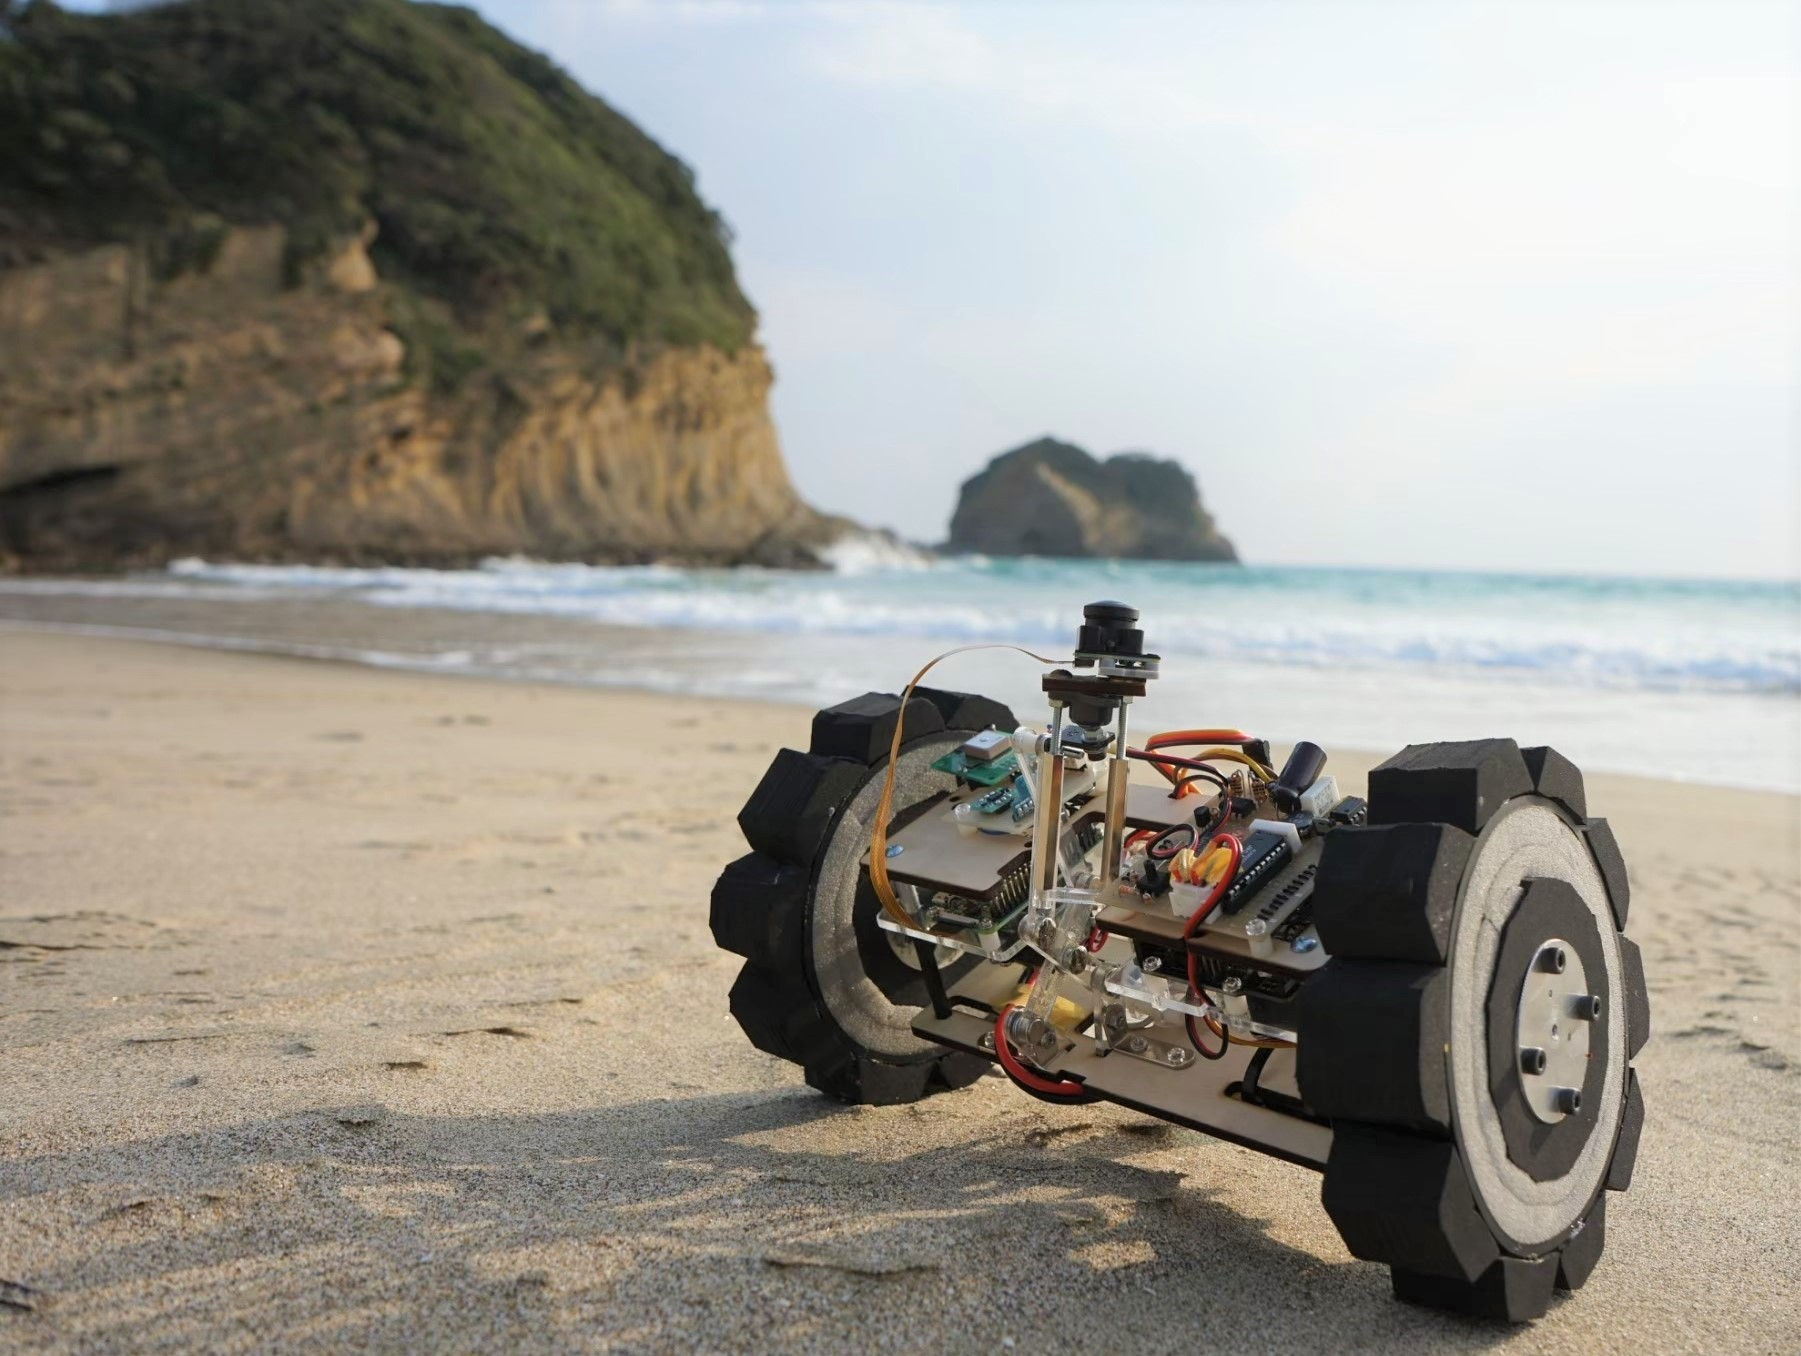
\includegraphics[width=0.8\linewidth]{cansat_sea}
		\end{minipage}
		\begin{minipage}{0.45\linewidth}
			主にCanSat(カンサット)と呼ばれる模擬人工衛星の開発を行い,毎年いくつかの大会に出場しています.その他にも宇宙・工学に関する基礎研究および応用研究,技術開発を取り扱い,文部科学省からも表彰頂いています.
		\end{minipage}
	\end{frame}
	
	\begin{frame}{「あかとき」はどんな団体か?}
		\begin{alertblock}{重要!!}
			世界で初めてXXした団体で,埼玉大学で唯一の宇宙工学を学べるところらしいです!
		\end{alertblock}
		\begin{block}{本当?}
			いろいろな野望を持ってチャレンジしていこう!
		\end{block}
		\begin{exampleblock}{例}
			おおお!!エネルギーがああああ!!
			\begin{equation}
				E = mc^2 , \quad \oint_c\mathbf E\cdot d\mathbf l=\int_s\left(-\frac{\partial\mathbf B}{\partial t}\right)\cdot d\mathbf S
			\end{equation}
		\end{exampleblock}
	\end{frame}

	\section{ChatGPTの「あかとき」の由来の考察}
	\begin{frame}{ChatGPT3.5の「あかとき」の由来の考察}
		
\includegraphics[width=1cm]{ChatGPT-Icon-Logo-PNG}
		\vspace{1em}
		
		「埼玉大学宇宙工学サークルあかとき」という団体の名前が「あかとき」と付けられた理由は、おそらく「あかとき」が明け方を表し、朝日が昇って新たな一日が始まることを意味することから、「\alert{新たな未来へ向かって発展する}」という願いが込められていると考えられます。また、「宇宙工学」に関連しているということもあり、「{\Large \color{blue}限界に挑戦する}」「{\Large \color{blue}新たな可能性を探求する}」という願いが込められていると思われます。
		\vspace{2em}
		\begin{alertblock}{Good Luck !!}
			応援してます
		\end{alertblock}
	\end{frame}
\end{document}